
\begin{figure}[H]
1. \textbf{Bolo ľahké sa zorientovať
v úvodnej obrazovke.}

Úvodná obrazovka by mala byť jasná a výstižná. Preto bolo potrebné zaviesť komponenty ako menu pre začiatok akcie či manipulácia s výslednými videami v úvodnej obrazovke tak, aby sa použivateľ vedeľ zorientovať bez určitých problémov.

Výsledok ukazuje, že použivatelia sa vedeli zorientovať v úvodnej obrazovke bez problémov. Tlačidlo pre menu vytvorenia videa bolo dosť zreteľné a intuitívne pre jeho výber. Výsledne videa v úvodnej obrazovke boli prehľadné. Avšak pre jedného uživateľa bol menší problém pri zorientovaní sa v otvorení menu pre akcie. Môže to byť spôsobené, nedostatočnou výstižnosťou ikony tlačidla.

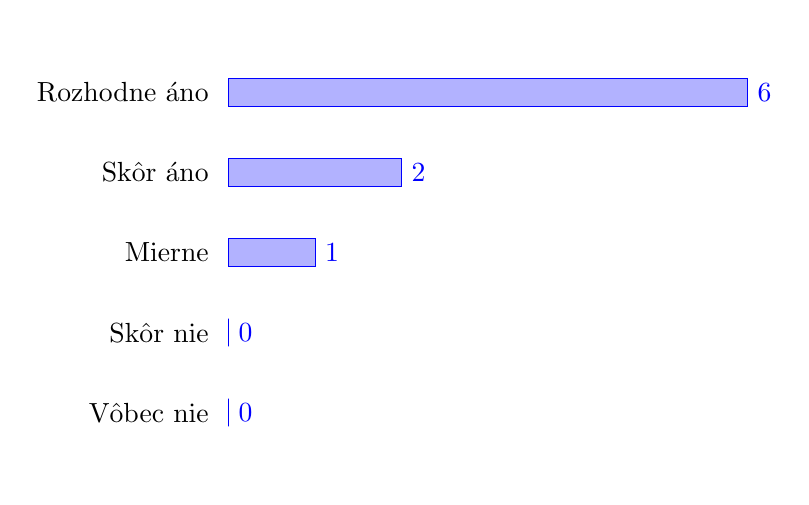
\begin{tikzpicture}
  \begin{axis}[title  = ,
    xbar,
    y axis line style = { opacity = 0 },
    axis x line       = none,
    tickwidth         = 0pt,
    enlarge y limits  = 0.2,
    enlarge x limits  = 0.02,
    symbolic y coords = { Vôbec nie, Skôr nie,Mierne, Skôr áno, Rozhodne áno},
    nodes near coords,
  ]
  \addplot coordinates { (6,Rozhodne áno)         (1,Mierne)
                         (2,Skôr áno)  (0,Skôr nie) (0,Vôbec nie)};

  \end{axis}

\end{tikzpicture}
\caption{Vyhodnotenie otázky - Bolo ľahké sa zorientovať
v úvodnej obrazovke.}
\end{figure}

\begin{figure}[H]
\textbf{2. Bolo ľahké si vybrať možnosť
pre začiatok vytvárania videa.}

Dôležitý proces aplikácie začiná práve pri výbere spôsobu spracovania videa, kde použivateľ má dve možnosti pri výbere vstupného súboru.

Výsledok ukazuje, že použivatelia si bez problémov vybrala spôsob spracovania.

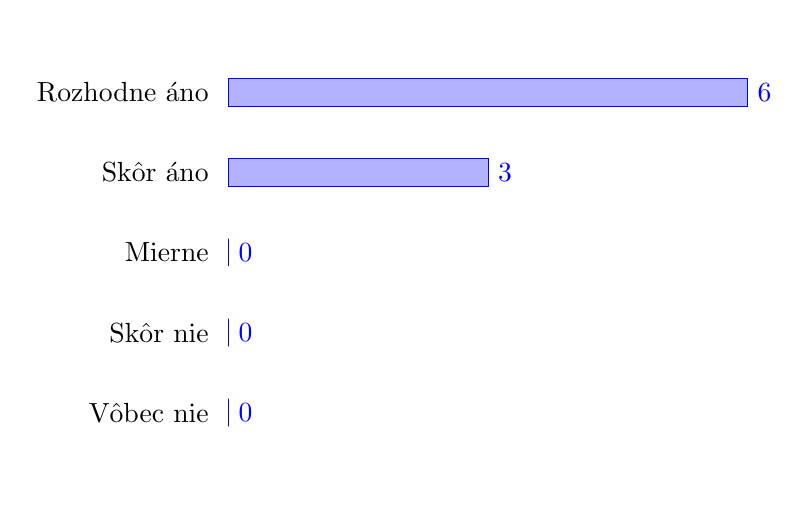
\begin{tikzpicture}
  \begin{axis}[title  = ,
    xbar,
    y axis line style = { opacity = 0 },
    axis x line       = none,
    tickwidth         = 0pt,
    enlarge y limits  = 0.2,
    enlarge x limits  = 0.02,
    symbolic y coords = { Vôbec nie, Skôr nie,Mierne, Skôr áno, Rozhodne áno},
    nodes near coords,
  ]
  \addplot coordinates { (6,Rozhodne áno)         (0,Mierne)
                         (3,Skôr áno)  (0,Skôr nie) (0,Vôbec nie)};

  \end{axis}
\end{tikzpicture}
\caption{Vyhodnotenie otázky - Bolo ľahké si vybrať možnosť
pre začiatok vytvárania videa.}
\end{figure}

\begin{figure}[H]
 \textbf{3. Náhľad kamery je úhľadný a
jednoduchý pre použitie.}

V tejto práci sme vytvorili svoj vlastný náhľad kamery priamo v aplikácií, kde boli implementované rôzne komponenty ako blest, otáčanie prednej a zadnej kamery, tlačidlo pre vybranie hudby na pozadie. Náhľad kamery sme sa snažili urobiť úhľadným spôsobom a preto sme všetky komponenty zakomponovali do priehľadného menu.


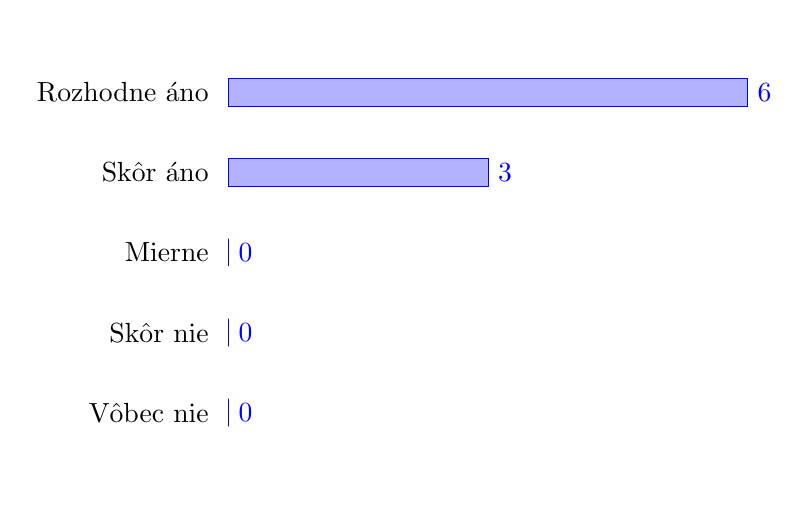
\begin{tikzpicture}
  \begin{axis}[title  =,
    xbar,
    y axis line style = { opacity = 0 },
    axis x line       = none,
    tickwidth         = 0pt,
    enlarge y limits  = 0.2,
    enlarge x limits  = 0.02,
    symbolic y coords = { Vôbec nie, Skôr nie,Mierne, Skôr áno, Rozhodne áno},
    nodes near coords,
  ]
  \addplot coordinates { (6,Rozhodne áno)         (0,Mierne)
                         (3,Skôr áno)  (0,Skôr nie) (0,Vôbec nie)};

  \end{axis}
\end{tikzpicture}
\caption{Vyhodnotenie otázky - Náhľad kamery je úhľadný a
jednoduchý pre použitie.}
\end{figure}



\begin{figure}[H]
\textbf{4. Vedel som sa zorientovať pre
výber hudby na pozadie.}

Touto otázkou sme sledovali to, či bolo tlačidlo alebo popis dostatočne zreteľný na to, aby použivateľ vedel vybrať hudbu na pozadie.

Pre viac ako polovicu uživateľov bola orientácia pri výbere hudby bez problémov. Oznámenie alebo tlačidlo pre výber hudby boli intuitívne pre použivateľa, avšak je treba ešte vylepšiť interakciu, aby použivateľ bol jasne oboznámený pre výber hudby.

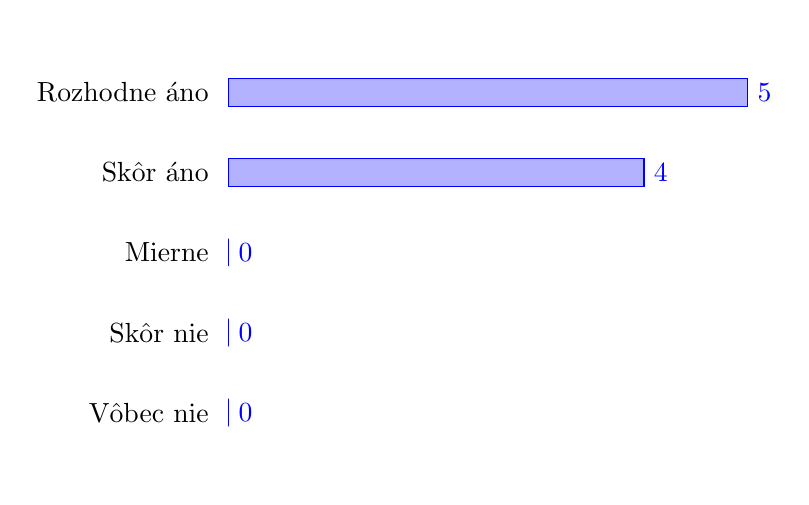
\begin{tikzpicture}
  \begin{axis}[title  = ,
    xbar,
    y axis line style = { opacity = 0 },
    axis x line       = none,
    tickwidth         = 0pt,
    enlarge y limits  = 0.2,
    enlarge x limits  = 0.02,
    symbolic y coords = { Vôbec nie, Skôr nie,Mierne, Skôr áno, Rozhodne áno},
    nodes near coords,
  ]
  \addplot coordinates { (5,Rozhodne áno)         (0,Mierne)
                         (4,Skôr áno)  (0,Skôr nie) (0,Vôbec nie)};

  \end{axis}
\end{tikzpicture}
\caption{Vyhodnotenie otázky - Vedel som sa zorientovať pre
výber hudby na pozadie.}
\end{figure}


\begin{figure}[H]
\textbf{5. Zoznam hudby bol prehľadný
a jeho výber bol jednoduchý.}

Keďže pri spracovaní videa je nutné si vybrať hudbu na pozadie, bolo nutné vytvoriť zoznam hudby jednoduchý pre jeho výber. Keďže použivateľ môže mať rôzne množstvo hudby v úložnom priestore zariadenia, bolo potrebné zistiť, či bol zoznam hudby prehľadný a výber jednoduchý.

Výsledky ukazujú, že komponent pre výber hudby splnil svoj účel a pre použivateľov bol daný zoznam hudby jednoduchý.

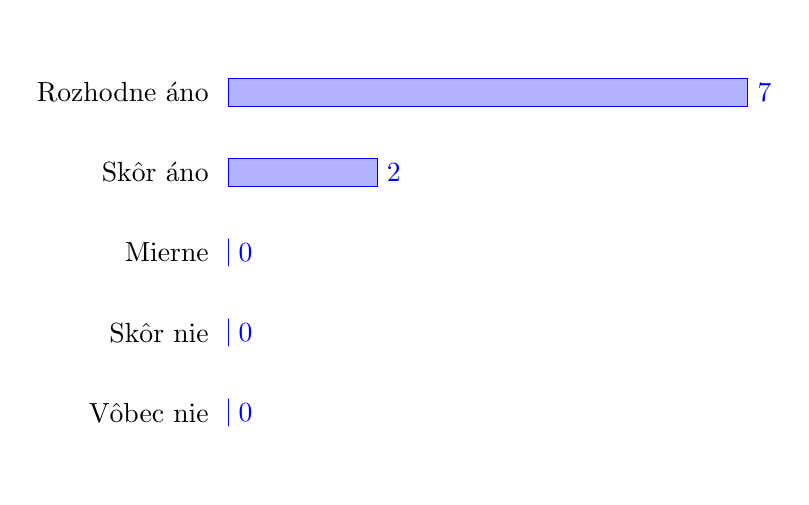
\begin{tikzpicture}
  \begin{axis}[title  = ,
    xbar,
    y axis line style = { opacity = 0 },
    axis x line       = none,
    tickwidth         = 0pt,
    enlarge y limits  = 0.2,
    enlarge x limits  = 0.02,
    symbolic y coords = { Vôbec nie, Skôr nie,Mierne, Skôr áno, Rozhodne áno},
    nodes near coords,
  ]
  \addplot coordinates { (7,Rozhodne áno)         (0,Mierne)
                         (2,Skôr áno)  (0,Skôr nie) (0,Vôbec nie)};

  \end{axis}
\end{tikzpicture}
\caption{Vyhodnotenie otázky - Zoznam hudby bol prehľadný
a jeho výber bol jednoduchý.}
\end{figure}


\begin{figure}[H]
\textbf{6. Bolo ľahké a nápomocné
zaznamenať video spolu s hudbou na pozadí.}

Touto otázkou sme sledovali, či zaznamenanie videa spolu s hudbou na pozadí bol účinný ale aj celý proces zaznamenávania kde zahŕňame náhľad kamery a výber hudby. 

Výsledky použivateľov ukazujú, že manipulácia s hudbou popri zaznamenávanie bola jednoduchá. Použivatelia vedeli zaznamenať video spolu s hudbou na pozadí, avšak nebola dostatočne zreteľná požiadavka pre výber hudby.

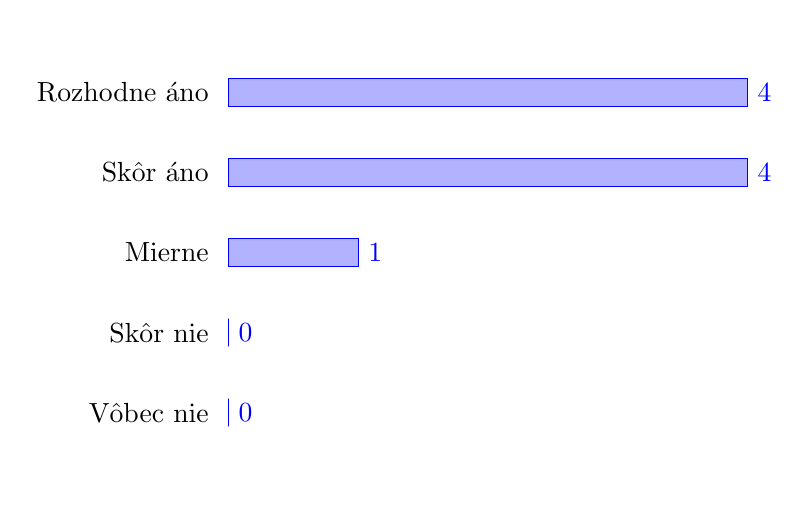
\begin{tikzpicture}
  \begin{axis}[title  = ,
    xbar,
    y axis line style = { opacity = 0 },
    axis x line       = none,
    tickwidth         = 0pt,
    enlarge y limits  = 0.2,
    enlarge x limits  = 0.02,
    symbolic y coords = { Vôbec nie, Skôr nie,Mierne, Skôr áno, Rozhodne áno},
    nodes near coords,
  ]
  \addplot coordinates { (4,Rozhodne áno)         (1,Mierne)
                         (4,Skôr áno)  (0,Skôr nie) (0,Vôbec nie)};

  \end{axis}
\end{tikzpicture}
\caption{Vyhodnotenie otázky - Bolo ľahké a nápomocné
zaznamenať video spolu s hudbou na pozadí.}
\end{figure}


\begin{figure}[H]
\textbf{7. Výber videa z galérie bol
jednoduchý a prehľadný.}

Použivateľ môže mať rôzny počet videí v úložnom priestore zariadenia. Bolo potrebné otestovať spôsob implementácie galérie poskytujúci priečinky v ktorých sú videa.

Spôsob implementovania výberu videa z galérie splnil svoj účel. Galéria je jednoduchá a plynulá aj pri väčšom množstve videí z úložného priestoru. Výber videa dopomohla hlavne implementácia priečinkov, pomocou ktorých použivateľ jasne indentifikoval kde sa daný súbor môže nachádzať.

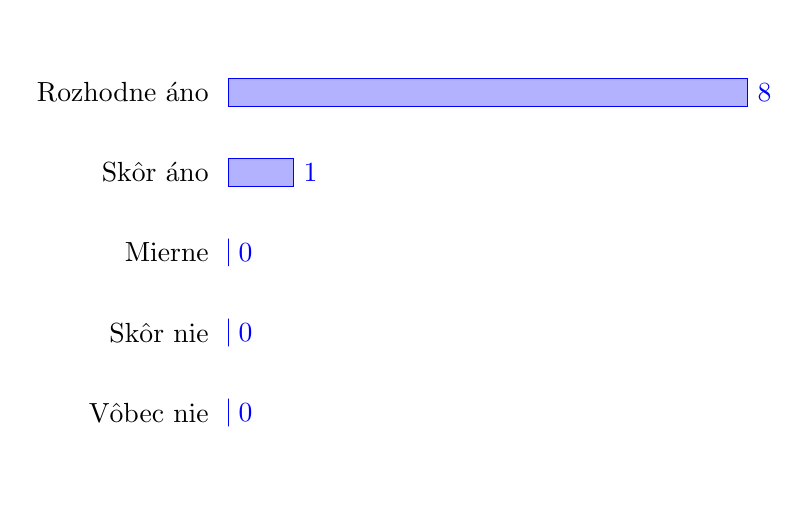
\begin{tikzpicture}
  \begin{axis}[title  = ,
    xbar,
    y axis line style = { opacity = 0 },
    axis x line       = none,
    tickwidth         = 0pt,
    enlarge y limits  = 0.2,
    enlarge x limits  = 0.02,
    symbolic y coords = { Vôbec nie, Skôr nie,Mierne, Skôr áno, Rozhodne áno},
    nodes near coords,
  ]
  \addplot coordinates { (8,Rozhodne áno)         (0,Mierne)
                         (1,Skôr áno)  (0,Skôr nie) (0,Vôbec nie)};

  \end{axis}
\end{tikzpicture}
\caption{Vyhodnotenie otázky - Výber videa z galérie bol
jednoduchý a prehľadný.}
\end{figure}


\begin{figure}[H]
\textbf{8. Spôsob orezania videa bol jednoduchý pre ovládanie.}
Existujú rozné spôsoby ako implementovať orezávanie videa. My sme na to použili knižnicu, pomocou ktorej vieme určiť úsek nového začiatku a konca videa. Chceli sme zistiť, ako naša implementácia funguje v praxi pri určení daného úseku.

Väčšina použivateľov rozhodne súhlasila akým spôsobom je možné orezávať video, avšak použivatelia by prijali možnosť orezávania pri otočení obrazovky na ležato. Týmto spôsobom by bolo oveľa jednoduchšie orezávanie videa pre použivateľov.

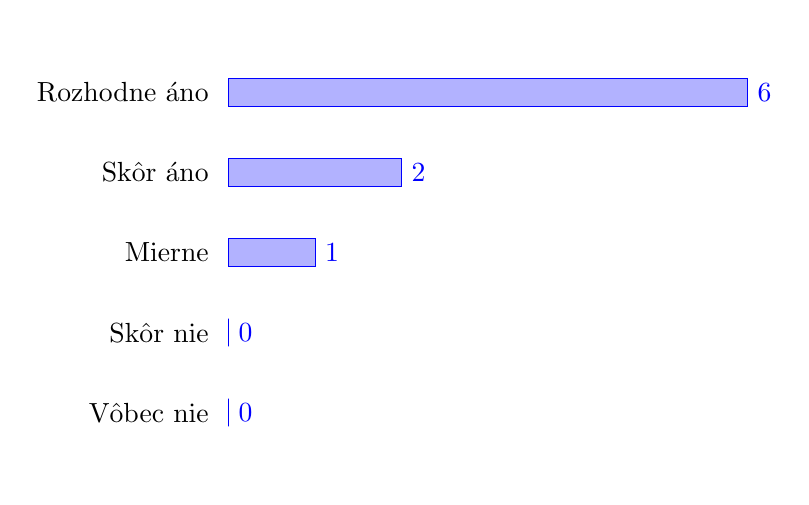
\begin{tikzpicture}
  \begin{axis}[title  = ,
    xbar,
    y axis line style = { opacity = 0 },
    axis x line       = none,
    tickwidth         = 0pt,
    enlarge y limits  = 0.2,
    enlarge x limits  = 0.02,
    symbolic y coords = { Vôbec nie, Skôr nie,Mierne, Skôr áno, Rozhodne áno},
    nodes near coords,
  ]
  \addplot coordinates { (6,Rozhodne áno)         (1,Mierne)
                         (2,Skôr áno)  (0,Skôr nie) (0,Vôbec nie)};

  \end{axis}
\end{tikzpicture}
\caption{Vyhodnotenie otázky - Spôsob orezania videa bol jednoduchý pre ovládanie.}
\end{figure}


\begin{figure}[H]
\textbf{9. Náhľad videa spracovaného pred samotným uložením vnímam ako prínos. }

Medzi najdôležitejšou funkcionalitou našej práce je náhľad videa. Preto sme chceli zistiť, ako je vnímaná naša funkcionalita alebo či mala pre použivateľov určitý prínos pri spracovaní videa.

Použivateľia ocenili funkcionalitu náhľadu videa v momente po spracovaní. Avšak samotný náhĺad možno nie je dostatnčne zreteľný pre uloženie či návrat na predošlú obrazovku. 
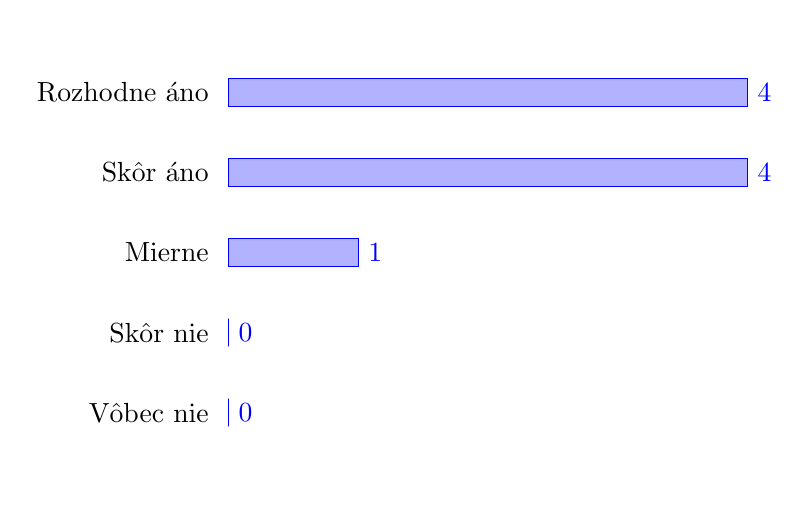
\begin{tikzpicture}
  \begin{axis}[title  = ,
    xbar,
    y axis line style = { opacity = 0 },
    axis x line       = none,
    tickwidth         = 0pt,
    enlarge y limits  = 0.2,
    enlarge x limits  = 0.02,
    symbolic y coords = { Vôbec nie, Skôr nie,Mierne, Skôr áno, Rozhodne áno},
    nodes near coords,
  ]
  \addplot coordinates { (4,Rozhodne áno)         (1,Mierne)
                         (4,Skôr áno)  (0,Skôr nie) (0,Vôbec nie)};

  \end{axis}
\end{tikzpicture}
\caption{Vyhodnotenie otázky - Náhľad videa spracovaného pred samotným uložením vnímam ako prínos.}
\end{figure}


\begin{figure}[H]
\textbf{10. Prechod medzi obrazovkami
bol jasný a plynulý.}

Mimo funkčnosti samotných komponentov bolo potrebné otestovať aj samotné správanie aplikácie. V tomto bode sme testovali hlavne funkčnosť animácií v prechode medzi obrazovkami. Taktiež sme testovali či bol prechod medzi obrazovkami dostatočne zreteľný pre použivateľa.

Prechod mezdi obrazovkami bol dostatočne zreteľný pre použivateľa. Pri tomto bode treba zohľadiť aj výkonnosť mobilného zariadenia, kde animácia a prechod nemuseli byť jasné a plynulé.

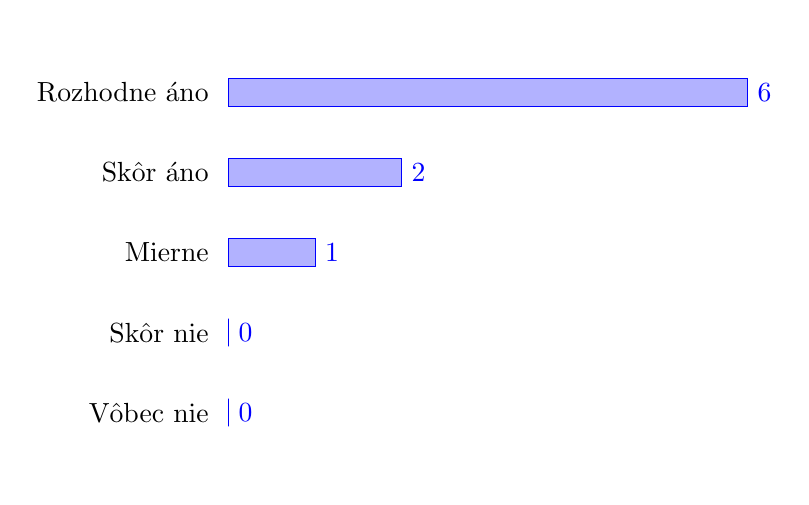
\begin{tikzpicture}
  \begin{axis}[title  = ,
    xbar,
    y axis line style = { opacity = 0 },
    axis x line       = none,
    tickwidth         = 0pt,
    enlarge y limits  = 0.2,
    enlarge x limits  = 0.02,
    symbolic y coords = { Vôbec nie, Skôr nie,Mierne, Skôr áno, Rozhodne áno},
    nodes near coords,
  ]
  \addplot coordinates { (6,Rozhodne áno)         (1,Mierne)
                         (2,Skôr áno)  (0,Skôr nie) (0,Vôbec nie)};

  \end{axis}
\end{tikzpicture}
\caption{Vyhodnotenie otázky - Prechod medzi obrazovkami
bol jasný a plynulý.}
\end{figure}


\begin{figure}[H]
\textbf{11. Proces uloženia videa na pozadí aplikácie vnímam ako prínos.}

Patrí to medzi najdôležitejšou funkcionalitou našej aplikácie. Proces uloženia videa na pozadí poskytuje použivateľovi flexibilitu používania a hlavne táto funkcionalita je šetrná pre batériu.

Väčšina použivateľov je nad mieru spokojná ohľadom prínosu, avšak je ešte potrebné zlepšiť, aby proces ukladania videa netrval veľmi dlho. Následne pri začiatku ukladania videa do zariadenia spustenie notifikácie nebolo dostatočne zreteľné.

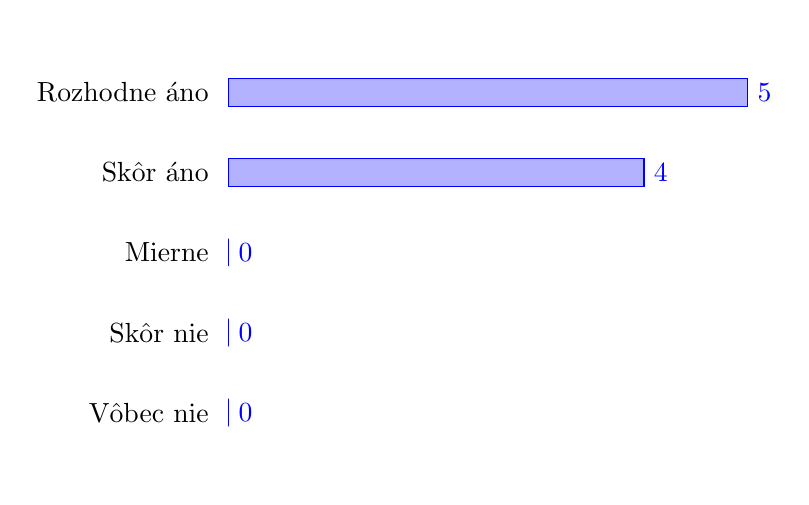
\begin{tikzpicture}
  \begin{axis}[title  = ,
    xbar,
    y axis line style = { opacity = 0 },
    axis x line       = none,
    tickwidth         = 0pt,
    enlarge y limits  = 0.2,
    enlarge x limits  = 0.02,
    symbolic y coords = { Vôbec nie, Skôr nie,Mierne, Skôr áno, Rozhodne áno},
    nodes near coords,
  ]
  \addplot coordinates { (5,Rozhodne áno)         (0,Mierne)
                         (4,Skôr áno)  (0,Skôr nie) (0,Vôbec nie)};

  \end{axis}
\end{tikzpicture}
\caption{Vyhodnotenie otázky - Proces uloženia videa na pozadí aplikácie vnímam ako prínos.}
\end{figure}


\begin{figure}[H]
\textbf{12. Bolo účinné prehrávanie a náhľad videa na celej obrazovke.}

Aplikáciu sme sa snažili vypracovať efektívne, čo znamená, aby sa aj obrazovka využila efektívne. Rozhodli sme sa maximalizovať obrazovku pre prehrávanie a tak sme chceli zistiť, či vďaka tomu bolo prehrávanie učinné.

Spôsob maximalizovania obrazovky účel pre používateľov splnil. Taktiež bolo prehrávaniu umožnené aj otáčanie obrazovky. Použivatelia boli spokojný so spôsobom ako sú implementované tlačidlá v rámci prehrávača na celej obrazovke.

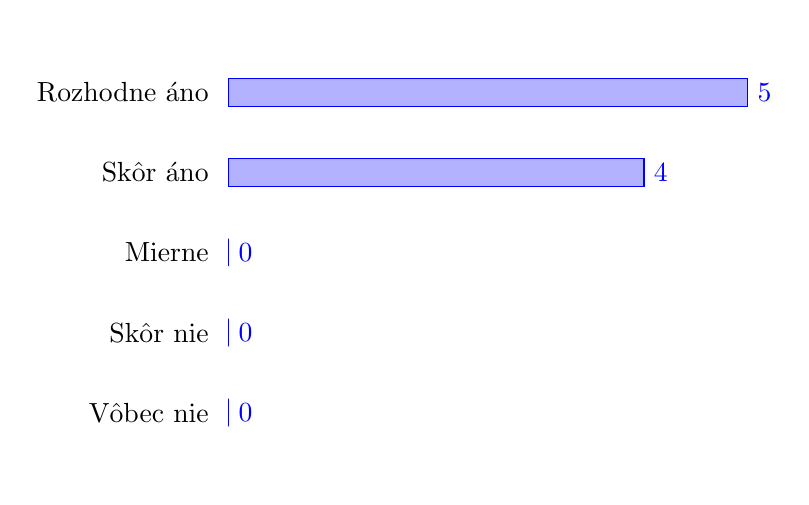
\begin{tikzpicture}
  \begin{axis}[title  = ,
    xbar,
    y axis line style = { opacity = 0 },
    axis x line       = none,
    tickwidth         = 0pt,
    enlarge y limits  = 0.2,
    enlarge x limits  = 0.02,
    symbolic y coords = { Vôbec nie, Skôr nie,Mierne, Skôr áno, Rozhodne áno},
    nodes near coords,
  ]
  \addplot coordinates { (5,Rozhodne áno)         (0,Mierne)
                         (4,Skôr áno)  (0,Skôr nie) (0,Vôbec nie)};

  \end{axis}
\end{tikzpicture}
\caption{Vyhodnotenie otázky - Bolo účinné prehrávanie a náhľad videa na celej obrazovke. }
\end{figure}


\begin{figure}[H]
\textbf{13. Navigácia a používanie aplikácie bolo intuitívne.}

Navigácia a aplikácie aplikácie znamená, či rozloženie komponentov na obrazovke a popis k nim bol dostatočne intuitívny na celkové používanie aplikácie.

Väčšina použivateľov nemala žiaden problem s používaním. Navigácia a používanie je intuitívne, avšak treba zohľadniť aj skúsenosti použivateľov s mobilnými technológiami.

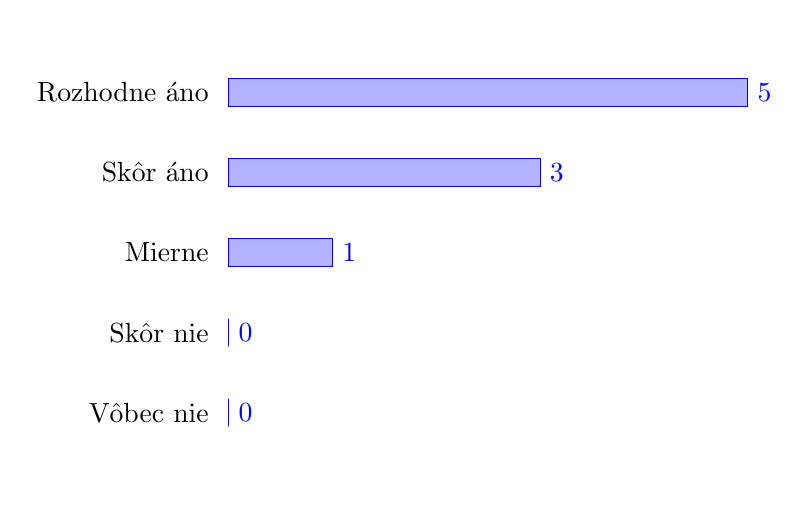
\begin{tikzpicture}
  \begin{axis}[title  = ,
    xbar,
    y axis line style = { opacity = 0 },
    axis x line       = none,
    tickwidth         = 0pt,
    enlarge y limits  = 0.2,
    enlarge x limits  = 0.02,
    symbolic y coords = { Vôbec nie, Skôr nie,Mierne, Skôr áno, Rozhodne áno},
    nodes near coords,
  ]
  \addplot coordinates { (5,Rozhodne áno)         (1,Mierne)
                         (3,Skôr áno)  (0,Skôr nie) (0,Vôbec nie)};

  \end{axis}
\end{tikzpicture}
\caption{Vyhodnotenie otázky - Navigácia a používanie aplikácie bolo intuitívne.}
\end{figure}


\begin{figure}[H]
 \textbf{14. Naučil som sa základne funkcie ako spracovať video počas tohto testovania.}
 
 Otázkou sme sledovali hlavne to, akým spôsobom sme implementovali celý proces spracovania videa. Celý proces by nemal byť zložitý pre používanie, čo znamená, že základné funkcie by nemali byť zložité pre ich používanie.
 
 Výsledky ukazujú jednoduchosť základných funkcií pri ktorých bolo zreteľné čo sa od nich očakáva. Avšak ešte existujú možnosti ako zjednodušiť základne funkcie ako napríklad umožnenie použivateľovi o menej klikov naviac na obrazovke.

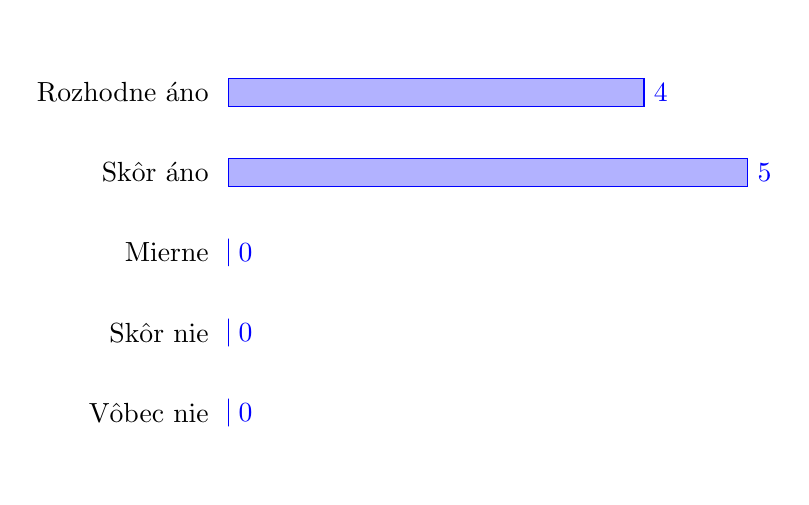
\begin{tikzpicture}
  \begin{axis}[title  =,
    xbar,
    y axis line style = { opacity = 0 },
    axis x line       = none,
    tickwidth         = 0pt,
    enlarge y limits  = 0.2,
    enlarge x limits  = 0.02,
    symbolic y coords = { Vôbec nie, Skôr nie,Mierne, Skôr áno, Rozhodne áno},
    nodes near coords,
  ]
  \addplot coordinates { (4,Rozhodne áno)         (0,Mierne)
                         (5,Skôr áno)  (0,Skôr nie) (0,Vôbec nie)};

  \end{axis}
\end{tikzpicture}
\caption{Vyhodnotenie otázky - Naučil som sa základne funkcie ako spracovať video počas tohto testovania.}
\end{figure}


\begin{figure}[H]
\textbf{15. Funkcie na obrazovkách boli jasne a zreteľné.}
 
Funkcie ako tlačidlo či ikona by mali byť dostatočne jasne a zreteľné na spôsob ich využívania. Funkcie na obrazovke by mali jasne reprezentovať to, čo sa od nich očakáva.

Použivatelia zhodnotili funkcie na obrazovke pozitívne. Ikony a popis k nim je dostatočne výstižný ich funkcionalite. Avšak určité funkcie možno neboli dostatočne výstižné napríklad pri uložení videa alebo hodnoty časov pri orezávani videa, kde pri hodnotách nie je uvedený popis.
 
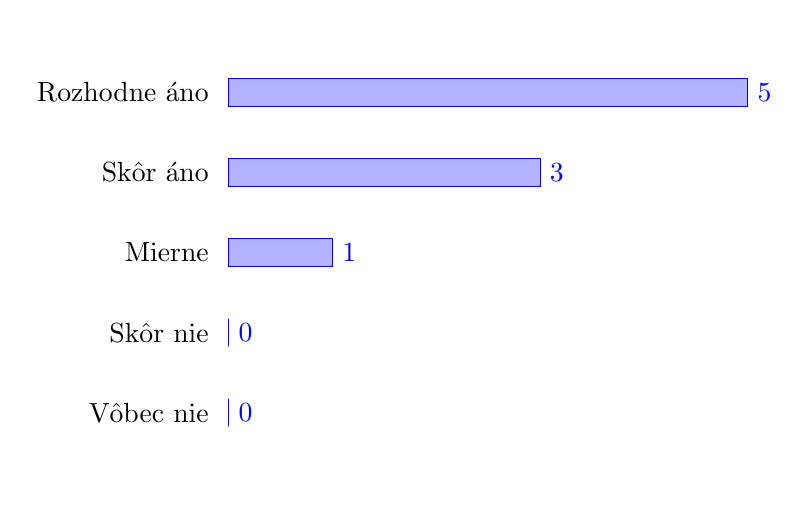
\begin{tikzpicture}
  \begin{axis}[title  =,
    xbar,
    y axis line style = { opacity = 0 },
    axis x line       = none,
    tickwidth         = 0pt,
    enlarge y limits  = 0.2,
    enlarge x limits  = 0.02,
    symbolic y coords = { Vôbec nie, Skôr nie,Mierne, Skôr áno, Rozhodne áno},
    nodes near coords,
  ]
  \addplot coordinates { (5,Rozhodne áno)         (1,Mierne)
                         (3,Skôr áno)  (0,Skôr nie) (0,Vôbec nie)};

  \end{axis}
\end{tikzpicture}
\caption{Vyhodnotenie otázky - Funkcie na obrazovkách boli jasne a zreteľné.}
\end{figure}


\begin{figure}[H]
\textbf{16. Aplikácia na efektívnu úpravu videa bola užitočná.}

Otázka bola mierená na výsledok aplikácie. Keďže našou úlohou tejto práce bolo vytvoriť aplikáciu na efektívnu úpravu videa, chceli sme zistiť, či naša aplikácia splnila použivateľov účel. 

Na výsledku tejto otázky môžeme vidieť, že cieľ našej práce sme splnili. Existuje ešte množnstvo spôsobov ako je možné túto aplikáciu vylepšiť. Použivatelia zhodnotili, že aplikácia bola užitočná.

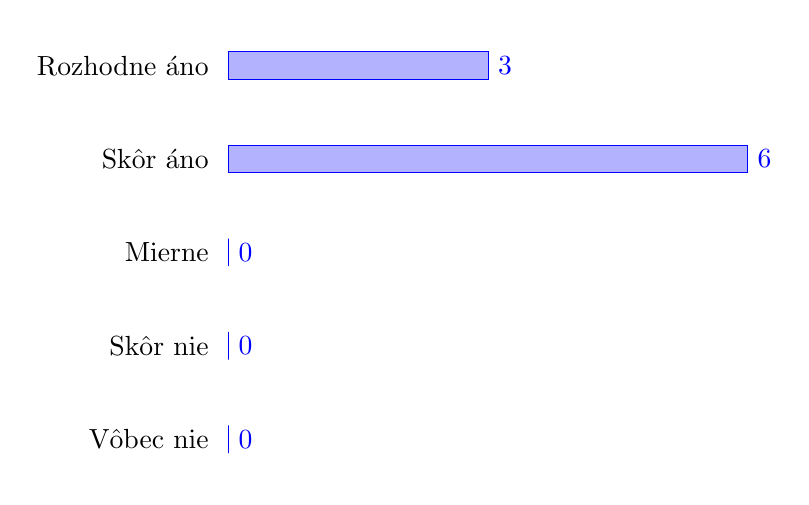
\begin{tikzpicture}
  \begin{axis}[title  = ,
    xbar,
    y axis line style = { opacity = 0 },
    axis x line       = none,
    tickwidth         = 0pt,
    enlarge y limits  = 0.1,
    enlarge x limits  = 0.02,
    symbolic y coords = { Vôbec nie, Skôr nie,Mierne, Skôr áno, Rozhodne áno},
    nodes near coords,
  ]
  \addplot coordinates { (3,Rozhodne áno)         (0,Mierne)
                         (6,Skôr áno)  (0,Skôr nie) (0,Vôbec nie)};

  \end{axis}
  
\end{tikzpicture}
\caption{Vyhodnotenie otázky - Aplikácia na efektívnu úpravu videa bola užitočná.}
\end{figure}


\begin{table}[H]
\centering
\begin{tabularx}{\textwidth}{
| >{\centering\arraybackslash}X
| >{\centering\arraybackslash}X
| >{\centering\arraybackslash}X |} 
\hline
\textbf{Odpovede} & \textbf{Počet výskytov} & \textbf{Percento} \\ 
\hline
Rozhodne áno                                    &               85                      &       59\%                        \\ \hline
Skôr áno                                        &                52                     &        36,1\%                       \\ \hline
Mierne                                          &                5                     &          3,5\%                     \\ \hline
Skôr nie                                        &                 2                    &          1,4\%                     \\ \hline
Vôbec nie                                       &                 0                    &            0\%                   \\ \hline
Celkovo                                         &                 144                    &          100\%                     \\ \hline


\end{tabularx}

\caption{Náhľad na vyhodnotenie prieskumu aplikácie. }
\end{table}

Treba zohľadniť skúsenosti použivateľa s aplikáciami ale aj výkonnosť zariadenia na ktorých používatelia vykonávali testy. Prieskum aplikácie možeme zhodnotiť úspešne. Použivatelia sa rýchlo naučili funkcionality, ktoré ponúka naša aplikácia. Zaznamenávanie či výber hudby bol pre nich jednoduchý a intuitívny. Náhľad videa spoločne s jeho uložením je prínosom pre účel testovatých použivateľov.

Avšak, dostali sme aj menej pozitívne hodnotenie. Ako napríklad strihanie videa, kde nie je možné otáčanie obrazovky. Určité tlačidla alebo popis k nim neboli dostatočné zreteľné, avšak je treba zohľadniť jazykovú bariéru, keďže naša aplikácia je vypracovaná v cudzom jazyku a nie každý ovláda anglický jazyk.



